\documentclass{beamer}
%%%%%%%%%%%%%%%%%%%%%%%%%%%%%%%%%%%%%%%%%%%%%%%%%%%%%%%%%%%%%%%%%%%%%%%%%%%%
\usepackage{bm}
\usepackage{amsmath}
\usepackage{amssymb}
\usepackage{microtype}
\usepackage{booktabs} % \toprule, \midrule, \bottomrule
%%% INCLUDE FILE FOR DEFINITIONS
%%% These may require various packages.

% Shortcuts in regular text
\newcommand{\degs}{\ensuremath{^\circ}}
\newcommand{\EE}[1]{\ensuremath{\times 10^{#1}}}
\newcommand{\ttimes}{\ensuremath{{}\times{}}}
\newcommand{\cclicense}{%
  \smash{\raisebox{-0.45ex}{%
  \setlength{\unitlength}{1em}%
  \begin{picture}(1,1)%
    \put(0.5,0.5){\circle{1}}
    \put(0.5,0.5){\hbox to 0pt{\hss\raisebox{-.45ex}{\tiny\textsf{CC}}\hss}}
  \end{picture}%
  }}%
  \hskip -1em%
  \href{http://creativecommons.org/licenses/by-nc-sa/3.0/}%
  {\ \hskip 1em \textsf{BY-NC-SA}}%
}

%\newcommand{\horizsep}{{\par\noindent\centering\rule[.25ex]{.75\columnwidth}{2pt}\par}}
\newcommand{\horizsep}{\vspace{\baselineskip}\noindent\hspace{\stretch{1}}$
\ast\qquad \ast\qquad \ast\qquad
$ \hspace{\stretch{1}} \vspace{\baselineskip}}
\newcommand{\pytrt}{\textsf{PyTRT}}

% Research
\newcommand{\lop}[1]{\mathcal{L}\!\left[#1\right]}
\newcommand{\lopinv}[2]{\mathcal{I}_{#1}\!\left[#2\right]}
\newcommand{\Dtens}{\mat{D}}
\newcommand{\Etens}{\mat{E}}
\newcommand{\Identitytens}{\mat{I}}
\newcommand{\APone}{AP$_1$}
\newcommand{\Pone}{P$_1$}
\newcommand{\SN}{S$_N$}%{S$_\text{N}$}%{$S_N$}%
\newcommand{\PN}{P$_N$}%{P$_\text{N}$}%{$P_N$}%
\newcommand{\CN}{Crank--Nicolson} %Yes, it's Nic not Nich
\newcommand{\Eddington}{\mathcal{E}} %whatever symbol I decided for Eddington
\newcommand{\RadEn}{E} %whatever symbol I decide for radiation energy
\newcommand{\Sigmatr}{\Sigma_{\mathit{tr}}}

% Program names
\newcommand{\cpp}{\textsf{C\raisebox{0.2ex}{++}}}

% General math shortcuts
\newcommand{\ud}{\mathop{}\!\mathrm{d}}
\newcommand{\pder}[2]{\frac{\partial #1}{\partial #2}}
\newcommand{\oder}[2]{\frac{\mathrm{d} #1}{\mathrm{d} #2}}
\newcommand{\tpder}[2]{{\partial #1}/{\partial #2}} %inlined
\newcommand{\toder}[2]{{\mathrm{d} #1}/{\mathrm{d} #2}} %inlined
\newcommand{\lra}{ \quad \Longrightarrow \quad }
\newcommand{\eexp}{\mathop{}\!\mathrm{e}} % upright ``e'' for exponent
\newcommand{\expp}[1]{\exp\!\left( {#1} \right)} % exp with parentheses
\newcommand{\qeq}{\stackrel{\mathrm{?}}{=}}

% Probability
\newcommand{\expectation}[1]{\mathop{}\!\mathrm{E}\!\left[ #1 \right]}
\DeclareMathOperator{\Var}{Var} % variance

% Asymptotic analysis
\DeclareMathOperator{\Ei}{Ei} % Exponential function
\newcommand{\lapl}[1]{\mathcal{L}[{#1}]} %laplace

%change the Re and Im operators from fancy curly letters
\DeclareMathOperator{\MathOpRe}{Re}
\renewcommand{\Re}{\MathOpRe}
\DeclareMathOperator{\MathOpIm}{Im}
\renewcommand{\Im}{\MathOpIm}

%imaginary ``i'' , upright 'i' or \imath
\newcommand{\iimag}{\mathrm{i}}

% Finite differences
\newcommand{\hot}{\text{h.o.t.}}
\newcommand{\inv}{^{-1}}

% Numerical Linear Algebra
\newcommand{\conj}{^{\ast}} % complex conjugate (transpose)
\newcommand{\norm}[1]{\left\| #1 \right\|} % double pipe
\newcommand{\abs}[1]{\left| #1 \right|} % single pipe
\newcommand{\eps}{\varepsilon}
\DeclareMathOperator{\fl}{fl}

\DeclareMathOperator{\acosh}{arccosh} 

% Define a command to write a nice-looking element, e.g. 4,2 He
\newcommand{\elem}[3]{\ensuremath{{}^{{#1}}_{{#2}}\mathrm{{#3}}}}

% Vector definitions
\newcommand{\mat}[1]{\mathbf{#1}} %matrix is bold upright
\renewcommand{\vec}[1]{\bm{#1}} %vector is bold italic
\newcommand{\op}[1]{\mathsf{#1}} % ``operator'' is sans serif

\newcommand{\vd}{\bm{\cdot}} % slightly bold vector dot
\newcommand{\del}{\vec{\nabla}} % gradient (Del) is bold
\newcommand{\grad}{\vec{\nabla}} % gradient

%\newcommand{\abr}[1]{\langle {#1} \rangle}
\newcommand{\abr}[1]{\left\langle {#1} \right\rangle} % angle brackets for avg.

%% topbox is useful in extended definitions of math terms inside an align
\newcommand{\topbox}[2][0.6]{\parbox[t]{#1\columnwidth}{\raggedright{}#2}}

% commands to make text in math mode appear as zero-width (better-looking
% integrals/sums, e.g.)
% from mathmode.pdf page 74, or Alexander R. Perlis ``A complement to \smash,
% \llap, and \rlap''

\def\mathllap{\mathpalette\mathllapinternal}
	\def\mathllapinternal#1#2{%
	\llap{$\mathsurround=0pt#1{#2}$}%
}
\def\clap#1{\hbox to 0pt{\hss#1\hss}}%
\def\mathclap{\mathpalette\mathclapinternal}%
\def\mathclapinternal#1#2{%
	\clap{$\mathsurround=0pt#1{#2}$}%
}
\def\mathrlap{\mathpalette\mathrlapinternal}%
\def\mathrlapinternal#1#2{%
	\rlap{$\mathsurround=0pt#1{#2}$}%
}

\definecolor{lightgray}{gray}{0.85}
%%%%%%%%%%%%%%%%%%%%%%%%%%%%%%%%%%%%%%%%%%%%%%%%%%%%%%%%%%%%%%%%%%%%%%%%%%%%

%30 minute presentation
%15 minutes scheduled for questions
%1 hour allotted total

\usetheme{AnnArbor}
\usecolortheme{seahorse}
\usecolortheme{orchid}
\usefonttheme[onlymath]{serif}
\setbeamercolor*{frametitle}{use=structure,bg=structure.fg!20!white}
\setbeamercolor*{frametitle right}{use=structure,bg=structure.fg!20!white}
\setbeamertemplate{navigation symbols}{\insertframenavigationsymbol}
\setbeamertemplate{caption}[numbered]

\title[ORNL Seminar]%
{An anisotropic diffusion approximation to nonlinear radiation transport}

\author[SRJ, EWL]{Seth~Johnson \and Ed~Larsen}

\institute[UMich]{
University of Michigan, Ann Arbor
}
\date[5/6/2011]{May 6, 2011}

\AtBeginSection[]
{
\begin{frame}
  \frametitle{Outline}
  \tableofcontents[currentsection]
\end{frame}
}

\hypersetup{colorlinks=true,linkcolor=black}

% only show section headings in table of contents
\setcounter{tocdepth}{1}

%use symbols for footnote
\renewcommand{\thefootnote}{\fnsymbol{footnote}}

\begin{document}
%%%%%%%%%%%%%%%%%%%%%%%%%%%%%%%%%%%%%%%%%%%%%%%%%%%%%%%%%%%%%%%%%%%%%%%%%%%%

\begin{frame}
\titlepage
\begin{center}
  
\includegraphics[width=0.2\textwidth]{../figures/umlogo}
\end{center}
\smash{
\includegraphics[width=0.2\textwidth]{../figures/neup-small}}
\end{frame}

%%%%%%%%%%%%%%%%%%%%%%%%%%%%%%%%%%%%%%%%%%%%%%%%%%%%%%%%%%%%%%%%%%%%%%%%%%%%
\section{Introduction}
%%%%%%%%%%%%%%%%%%%%%%%%%%%%%%%%%%%%%%%%
\begin{frame}
  \frametitle{Thermal radiative transfer}
  \begin{itemize}
    \item TRT is the dominant heat transfer process in very hot materials
    \item Photons born isotropically via black body emission
      ($q_\text{rad} \propto \sigma T^4$)
    \item Cold material heats up and becomes relatively transparent
      ($\sigma\propto T^{-3}$)
  \end{itemize}

  Difficulties in solving:
  \begin{itemize}
    \item High dimensionality of solution phase space $(\vec{x}, \vec{\Omega},
      h\nu, t)$
    \item Highly nonlinear coupled partial differential equations for radiation
      field $\psi(\vec{x}, \vec{\Omega}, h\nu, t)$ and material energy
  \end{itemize}

  Particular application of this work: CRASH project
  \begin{itemize}
    \item Center for RAdiative Shock Hydrodynamics program: ``Assessment
      of Predictive Capability''
    \item Simulate laser-driven shock in a xenon-filled tube
    \item Uncertainty quantification: hundreds of solution instances needed
  \end{itemize}
\end{frame}

%%%%%%%%%%%%%%%%%%%%%%%%%%%%%%%%%%%%%%%%
\begin{frame}
  \frametitle{Motivation}
\begin{center}
  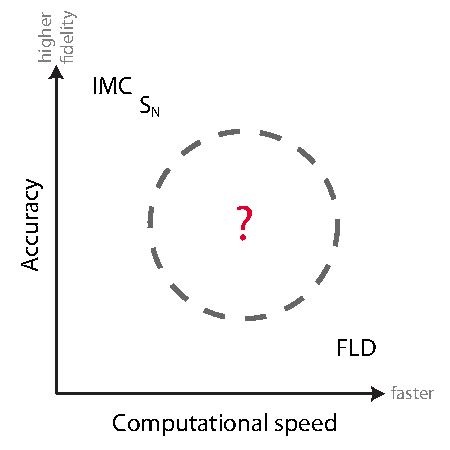
\includegraphics[width=3in]{../figures/fidelity}
\end{center}
% also, storage requirements
\end{frame}

%%%%%%%%%%%%%%%%%%%%%%%%%%%%%%%%%%%%%%%%
\begin{frame}
  \frametitle{Gray TRT equations}
  Common approximations for radiation transport methods development:
  \begin{itemize}
    \item work in a fixed medium, disregarding material advection;
    \item assume local thermodynamic equilibrium (LTE), which uses a single
      material temperature;
    \item neglect thermal conduction in material;
    \item average over all photon energies $h\nu$ (gray).
  \end{itemize}
\begin{subequations} \label{eqs:fullGrayTRT}
  Radiation transfer equation, angular flux $\psi(\vec{x}, \vec{\Omega}, t)$:
\begin{equation} \label{eq:fullGrayTransport}
  \frac{1}{c} \pder{\psi}{t}
  + \vec{\Omega} \vd \del \psi +
 \sigma \psi
  = \frac{\sigma c aT^4}{4\pi} 
  + \frac{c Q}{4\pi}
\end{equation}
  Material energy balance equation:
\begin{equation} \label{eq:fullGrayMaterial}
  \frac{1}{c_v}\pder{T}{t} = \sigma \int_{4\pi}  \psi \ud\Omega - \sigma c aT^4
\end{equation}
\end{subequations}
\end{frame}

%%%%%%%%%%%%%%%%%%%%%%%%%%%%%%%%%%%%%%%%
\begin{frame}
  \frametitle{Anisotropic diffusion}
  Previous work:
  \begin{itemize}
    \item Steady-state infinite medium VHTR-like problem with analytically
      calculated coefficients \cite{Lar2009c}
    \item Non-local tensor diffusion \cite{Mor2007} for steady-state
      radiative transfer, no further development or analysis in literature
  \end{itemize}
  Current work:
  \begin{itemize}
    \item Formulates boundary conditions and time-dependent terms
    \item Uses transport-calculated anisotropic diffusion tensors
    \item Applies to nonlinear, time-dependent problems with isotropic sources
  \end{itemize}
  Potential applications:
  \begin{itemize}
    \item Extends diffusion theory to new regimes of applicability
    \item Variance reduction with shielding problems that have voids
  \end{itemize}
\end{frame}

%%%%%%%%%%%%%%%%%%%%%%%%%%%%%%%%%%%%%%%%%%%%%%%%%%%%%%%%%%%%%%%%%%%%%%%%%%%%
\section{Theory}
\subsection{Summary in advance}
%%%%%%%%%%%%%%%%%%%%%%%%%%%%%%%%%%%%%%%%
\begin{frame}
\begin{enumerate}
  \item Define the anisotropic angular flux as $\Psi = \psi -
    \frac{1}{4\pi}\phi$. To handle boundary conditions, define $\Psi
    \equiv \tilde \Psi + \Psi_\mathrm{bl}$. We will approximate $\tilde \Psi$
    rather than $\psi$, and use $\Psi_\mathrm{bl}$ to determine matched boundary
    conditions.
  \item From the radiation transport equation and conservation equation, we get
    a differential transport equation for $\tilde \Psi$ and $\Psi_\mathrm{bl}$.
    Transform the former to an \emph{integral} transport equation for $\tilde
    \Psi$.
  \item Assume $\psi=O(1)$, $\frac1c\pder{}{t}=O(\epsilon^2)$, $\grad =
    O(\epsilon)$, $\int_{4\pi} \vec{\Omega} (\cdot) \ud\Omega = O(\epsilon)$.
  \item Use Taylor series to approximate nonlocal unknowns with local
    unknowns, discarding small terms. This yields
    \begin{equation*}
      \tilde \Psi(\vec{x}, \vec{\Omega})
      \approx - f(\vec{x}, \vec{\Omega})  \vec{\Omega} \vd \grad \phi\,.
    \end{equation*}
  \item Apply standard transport-matching procedure to $\Psi_\mathrm{bl}$. Use
    the identity $\int_{4\pi} \Psi \ud\Omega=0$ to find the boundary condition
    for $f$.
  \item Take the first angular moment of $\tilde \Psi$ to get
    $\vec{J}=-\Dtens \vd \grad \phi$
  \item Substitute $\vec{J}$ into the time-dependent particle
    conservation equation to get time-dependent anisotropic diffusion.
\end{enumerate}
\end{frame}

\subsection{Transport}
%%%%%%%%%%%%%%%%%%%%%%%%%%%%%%%%%%%%%%%%
\begin{frame}{Transport equation}
  Inside a time step, with ``frozen'' cross sections (opacities):
\begin{subequations} \label{eqs:fullTransport}
\begin{multline} \label{eq:fullTransportVol}
  \frac{1}{c} \pder{\psi}{t}(\vec{x}, \vec{\Omega}, t)
    + \vec{\Omega}\vd \grad \psi(\vec{x}, \vec{\Omega}, t)
    + \sigma^\ast(\vec{x}) \psi (\vec{x}, \vec{\Omega}, t)
    \\
    = \frac{1}{4\pi} \sigma^\ast(\vec{x}) ac [T(\vec{x}, t)]^4
    + \frac{1}{4\pi} q_{r}(\vec{x}, t)
    \equiv \frac{1}{4\pi} Q(\vec{x}, t) \,,
\\
x \in V,\  0 \le t < \Delta_t, \ \vec{\Omega} \in 4\pi,
\end{multline}
with the boundary condition
\begin{equation} \label{eq:fullTransportBndy}
  \psi(\vec{x}, \vec{\Omega}, t) = \psi^b(\vec{x}, \vec{\Omega}, t) \,,
 \quad \vec{x} \in \partial V, \ \vec{\Omega} \vd \vec{n} < 0,\ 0 \le t < \Delta_t
\end{equation}
and the initial condition
\begin{equation} \label{eq:fullTransportInit}
 \psi(\vec{x}, \vec{\Omega}, 0) = \psi^i(\vec{x}, \vec{\Omega}, t) \,,
 \quad \vec{x} \in V, \ \vec{\Omega} \in 4\pi\,.
\end{equation}
\end{subequations}
\end{frame}

%%%%%%%%%%%%%%%%%%%%%%%%%%%%%%%%%%%%%%%%
\begin{frame}{Conservation equations}
Operating on Eq.~\eqref{eq:fullTransportVol} by $\int_{4\pi} (\cdot) \ud\Omega$
gives
\begin{subequations} \label{eqs:loEquations}
\begin{equation} \label{eq:loVol}
\frac{1}{c} \pder{\phi}{t} (\vec{x}, t)
  + \grad \vd\vec{J}(\vec{x}, t)
  + \sigma^\ast \phi(\vec{x}, t)
  =  Q(\vec{x}, t)\,.
\end{equation}
and on the initial condition, Eq.~\eqref{eq:fullTransportInit},
\begin{equation} \label{eq:loInit}
\phi(\vec{x}, 0) = \int_{4\pi}  \psi^i(\vec{x},
\vec{\Omega}) \ud\Omega = \phi^i(\vec{x}) \,.
\end{equation}
\end{subequations}

Add $\vec{\Omega}\vd\grad \phi$ to both sides of Eq.~\eqref{eq:loVol} and
multiply by $\frac{1}{4\pi}$:
\begin{equation} \label{eq:modifiedConservation}
  \frac{1}{4\pi} \frac{1}{c} \pder{\phi}{t}
  + \frac{1}{4\pi} \vec{\Omega}\vd\grad \phi
  + \frac{1}{4\pi} \sigma^\ast \phi
  = \frac{1}{4\pi}  Q(\vec{x}, t) + \frac{1}{4\pi} \vec{\Omega}\vd\grad \phi
  - \frac{1}{4\pi} \grad \vd\vec{J}
\end{equation}
\end{frame}

\subsection{Anisotropic Transport}
%%%%%%%%%%%%%%%%%%%%%%%%%%%%%%%%%%%%%%%%
\begin{frame}{Anisotropic angular flux equations}
  Define ``anisotropic angular flux'':
  \begin{equation} \label{eq:capPsi}
    \Psi(\vec{x}, \vec{\Omega}) \equiv \psi(\vec{x}, \vec{\Omega})
    - \frac{1}{4\pi} \phi(\vec{x})\,.
  \end{equation}
  (This satisfies $\int_{4\pi} \Psi=0$ and $\int_{4\pi} \vec{\Omega} \Psi =
  \vec{J}$.)

  Subtract Eq.~\eqref{eq:modifiedConservation} from
  Eq.~\eqref{eq:fullTransportVol}; the isotropic source cancels:
\begin{multline*}
  \frac{1}{c} \pder{}{t} \left[ \psi - \frac{\phi}{4\pi} \right]
    + \vec{\Omega}\vd \grad \left[ \psi - \frac{\phi}{4\pi} \right]
    + \sigma^\ast(\vec{x})\left[ \psi - \frac{\phi}{4\pi} \right]
  = \frac{1}{4\pi} \grad \vd\vec{J} -
  \frac{1}{4\pi} \vec{\Omega}\vd \grad \phi
\end{multline*}

  Subtract $\phi/4\pi$ from the transport boundary condition:
  %($\vec{x} \in \partial V$, $\vec{\Omega} \vd \vec{n} < 0$):
  \begin{equation*}
    \psi - \frac{\phi}{4\pi} = \psi^b - \frac{\phi}{4\pi}
  \end{equation*}

  Subtract Eq.~\eqref{eq:loInit} from Eq.~\eqref{eq:fullTransportInit}:
  \begin{equation*}
    \psi(\vec{x}, \vec{\Omega}, 0) - \frac{1}{4\pi}\phi(\vec{x}, 0)
    = \psi^i - \frac{\phi^i}{4\pi}
  \end{equation*}
\end{frame}

%%%%%%%%%%%%%%%%%%%%%%%%%%%%%%%%%%%%%%%%
\begin{frame}{Anisotropic angular flux equations}
  Transport equation:
\begin{equation*}
  \frac{1}{c} \pder{}{t} \Psi
   + \vec{\Omega}\vd \grad \Psi
   + \sigma^\ast(\vec{x}) \Psi
  = \frac{1}{4\pi} \grad \vd\vec{J} -
  \frac{1}{4\pi} \vec{\Omega}\vd \grad \phi
  \equiv \hat Q(\vec{x}, \vec{\Omega}, t)
\end{equation*}

  Boundary condition:
  \begin{equation*}
    \Psi = \Psi^b = \psi^b - \frac{\phi}{4\pi}
  \end{equation*}

  Initial condition:
  \begin{equation*}
    \Psi(\vec{x}, \vec{\Omega}, 0) = \Psi^i = \psi^i - \frac{\phi^i}{4\pi} \,.
  \end{equation*}

  The exact solutions for $\psi$, $\phi$, $\vec{J}$ satisfy these equations: still
  no approximations.
\end{frame}

%%%%%%%%%%%%%%%%%%%%%%%%%%%%%%%%%%%%%%%%
\begin{frame}{Boundary layer equations}
In anticipation of approximating $\tilde \Psi = - f \vec{\Omega}\vd \grad \phi$,
separate $\Psi$ into a boundary layer plus an internal solution:
\begin{equation*}
  \Psi(\vec{x}, \vec{\Omega}, t)
  \equiv \tilde \Psi(\vec{x}, \vec{\Omega}, t)
  + \Psi_\mathrm{bl}(\vec{x}, \vec{\Omega}, t)\,.
\end{equation*}
The exact equations for $\tilde \Psi$:
\begin{equation*}
  \frac{1}{c} \pder{}{t} \tilde\Psi
   + \vec{\Omega}\vd \grad \tilde\Psi
   + \sigma^\ast(\vec{x}) \tilde\Psi
  =  \hat Q(\vec{x}, \vec{\Omega}, t)
\end{equation*}
with new boundary condition for $\vec{x} \in \partial V$, $\vec{\Omega}\vd
\vec{n} < 0$:
\begin{equation*}
  \tilde\Psi = -\zeta \vec{\Omega}\vd \grad \phi\,.
\end{equation*}

Therefore the corresponding boundary layer equation is:
\begin{equation*}
  \frac{1}{c} \pder{}{t} \Psi_\mathrm{bl}
   + \vec{\Omega}\vd \grad \Psi_\mathrm{bl}
   + \sigma^\ast(\vec{x}) \Psi_\mathrm{bl}
  = 0
\end{equation*}
with boundary condition for $\vec{x} \in \partial V$, $\vec{\Omega}\vd
\vec{n} < 0$:
\begin{equation*}
  \Psi_\mathrm{bl} = \psi^b - \frac{1}{4\pi} \phi + \zeta \vec{\Omega}\vd \grad
  \phi \,.
\end{equation*}

{\small Still no approximations.}
\end{frame}

%%%%%%%%%%%%%%%%%%%%%%%%%%%%%%%%%%%%%%%%
\begin{frame}{Integral transport equation}
  Streaming path from $(\vec{x}, t)$ backward along $-\vec{\Omega}$, accumulate
  sources and attenuate:
\begin{subequations} \label{eqs:inverseTransport}
  \begin{align} \label{eq:inverseTransportFull}
  \begin{split}
    \tilde \Psi(\vec{x}, \vec{\Omega}, t)
    &=
    \tilde \Psi^b(\vec{x} - s_b\vec{\Omega}, \vec{\Omega}, t - s_b/c)
    \eexp^{ -\tau(\vec{x}, \vec{x} - s_b \vec{\Omega})}
    U(ct - s_b)
    \\
    &\qquad + \Psi^i( \vec{x} - ct \vec{\Omega}, \vec{\Omega})
    \eexp^{ -\tau(\vec{x}, \vec{x} - ct \vec{\Omega})}
    U( s_b - ct)
    \\
    &\qquad + \int_{0}^{s_b}
    \left[ \hat Q(\vec{x} - s \vec{\Omega}, \vec{\Omega}, t-s/c)
    \right]
    \eexp^{ -\tau(\vec{x}, \vec{x} - s \vec{\Omega})}
    \ud s\,.
  \end{split}
    \\ 
    &\equiv \lopinv{b}{\tilde \Psi^b}
    + \lopinv{i}{\Psi^i}
    + \lopinv{v}{\hat Q} 
  \end{align}
  $s_b$ is the distance to the boundary, $U(\cdots)$ is the heaviside function,
  and the optical thickness is 
  \begin{equation} \label{eq:fullTauDefinition}
    \tau(\vec{x}, \vec{x}') = \int_{0}^{\norm{\vec{x} -
    \vec{x}'}} \sigma^\ast(\vec{x}-s\vec{\Omega}) \ud s \,.
  \end{equation}
\end{subequations}
These are nonlocal unknowns; we will approximate them with local unknowns.
\end{frame}

\subsection{Approximations}
%%%%%%%%%%%%%%%%%%%%%%%%%%%%%%%%%%%%%%%%
\begin{frame}{Time for some approximations}
  Asymptotic ansatz: assume weak spatial gradients, mildly anisotropic angular flux, very small time
  derivative:
\begin{align*}
  \psi &= O(1), &
  \del \psi &= O(\epsilon)&
  \int_{4\pi} \vec{\Omega} \psi\ud\Omega &= O(\epsilon)&
  \frac{1}{c} \pder{}{t} &= O(\epsilon^2)
\end{align*}

Our first approximation: $\lopinv{i}{\cdot} = O(\epsilon^2)$ and $\grad \vd \vec{J} =
O(\epsilon^2)$:
\begin{align*}
  \tilde \Psi &=
  \lopinv{i}{\Psi^i}
  - \lopinv{b}{\zeta\vec{\Omega}\vd \grad \phi}
  + \lopinv{v}{\frac{1}{4\pi} \grad \vd\vec{J}} -
  \lopinv{v}{\frac{1}{4\pi} \vec{\Omega}\vd \grad \phi}
    \\ 
  \tilde \Psi 
  &\approx -\lopinv{b}{\zeta\vec{\Omega}\vd \grad \phi}
  - \lopinv{v}{\frac{1}{4\pi} \vec{\Omega}\vd \grad \phi}
  + O(\epsilon^2)
\end{align*}

Taylor series expansion:
\begin{align} \nonumber
  \phi(\vec{x} - s\vec{\Omega}, t - s/c)
  &\sim \phi(\vec{x}, t)
  - s \bigg( \frac{1}{c} \pder{}{t} + \vec{\Omega} \vd \grad \bigg)
  \phi(\vec{x}, t) + O(\epsilon^2)
\\ \label{eq:taylorPhi}
\phi(\vec{x} - s\vec{\Omega}, t - s/c)
&= \phi(\vec{x}, t) + O(\epsilon)
\end{align}
\end{frame}

%%%%%%%%%%%%%%%%%%%%%%%%%%%%%%%%%%%%%%%%
\begin{frame}{Taylor series applied}
  If $\phi$ is smooth like the ansatz hypothesizes, the volumetric term becomes:
  \begin{align} \nonumber
  -\lopinv{v}{ \frac{1}{4\pi} \vec{\Omega}\vd \grad \phi }
  &= -\int_{0}^{s_b}
    \left[ \frac{1}{4\pi} \vec{\Omega}\vd \grad \phi \right]_{(\vec{x} - s
    \vec{\Omega}, t-s/c)}
    \eexp^{ -\tau(\vec{x}, \vec{x} - s \vec{\Omega})}
    \ud s
  \\\nonumber
  &\sim - \int_{0}^{s_b}
    \left[ \frac1{4\pi}\right]
    \eexp^{ -\tau(\vec{x}, \vec{x} - s \vec{\Omega})} \ud s
    \vec{\Omega}\vd \grad \phi(\vec{x},t) + O(\epsilon^2)
  \\\label{eq:tildeS}
  &= - \lopinv{v}{ \frac1{4\pi} } \vec{\Omega}\vd \grad \phi(\vec{x},t)\,.
  \end{align}
  The boundary term similarly is
  \begin{align} \nonumber
  - \lopinv{b}{ \zeta \vec{\Omega}\vd \grad \phi }
  &= -\int_{0}^{s_b}
    \left[\zeta \vec{\Omega}\vd \grad \phi \right]_{(\vec{x} - s_b
    \vec{\Omega}, t-s_b/c)}
    \eexp^{ -\tau(\vec{x}, \vec{x} - s \vec{\Omega})}
    \ud s
  \\ \label{eq:tildeB}
  &\sim - \lopinv{b}{ \zeta }
  \vec{\Omega}\vd \grad \phi(\vec{x},t)\,.
  \end{align}
  Thus,
  \begin{equation}\label{eq:capPsiApprox}
    \tilde\Psi(\vec{x}, \vec{\Omega}, t) \approx
    - \left[ \lopinv{b}{ \zeta }
    + \lopinv{v}{ \frac1{4\pi} } \right]
    \vec{\Omega}\vd \grad \phi(\vec{x},t)
    \equiv -f(\vec{x}, \vec{\Omega}) \vec{\Omega}\vd \grad \phi(\vec{x},t)
  \end{equation}
\end{frame}

\subsection{Boundary layer analysis}
%%%%%%%%%%%%%%%%%%%%%%%%%%%%%%%%%%%%%%%%
\begin{frame}{Transport matched boundary}
  Transport theory: boundary solution decays quickly if we enforce the relation
  $0 = \int_{\vec{\Omega}\vd \vec{n} < 0} W(\abs{\vec{\Omega}\vd \vec{n}})
  \Psi_\mathrm{bl} \ud\Omega$ on the boundary, where $W(\mu) \approx 2 \mu + 3
  \mu^2$ is related to the Chandrasekhar function. The transport extrapolation
  distance is $\int_0^1 \mu W \ud \mu / \int_0^1 W \ud \mu$.
  \begin{align*}
  0
  &= \int_{\vec{\Omega}\vd \vec{n} < 0} W(\abs{\vec{\Omega}\vd \vec{n}})
  \Psi_\mathrm{bl} \ud\Omega
  \\
  &= \int_{\vec{\Omega}\vd \vec{n} < 0} W \left[ \psi^b
  - \frac{1}{4\pi} \phi
  + \zeta \vec{\Omega} \vd \grad \phi \right] \ud\Omega
  \end{align*}
  or
  \begin{equation} \label{eq:loBndy}
  \int_{\vec{\Omega}\vd \vec{n} < 0} W \psi^b \ud\Omega
  = \phi - \int_{\vec{\Omega}\vd \vec{n} < 0} W \zeta \vec{\Omega} \ud\Omega
  \vd \grad \phi
  \end{equation}
  One more equation is needed to determine $\zeta$.
\end{frame}

%%%%%%%%%%%%%%%%%%%%%%%%%%%%%%%%%%%%%%%%
\begin{frame}{Determining $\zeta$}
 Recall that in the exact anisotropic transport equation,
 $\int_{4\pi}\Psi\ud\Omega = 0$. So we choose to
 enforce $\int_{4\pi}\tilde\Psi\ud\Omega = 0$ on the boundary:
 \begin{equation*}
   0 = \int_{4\pi} \tilde\Psi\ud\Omega
   = \int_{\vec{\Omega}\vd \vec{n} < 0} \left(
   -\zeta\vec{\Omega}\vd \grad \phi \right)\ud\Omega
   + \int_{\vec{\Omega}\vd \vec{n} > 0} \left(
   - f \vec{\Omega}\vd \grad \phi \right)\ud\Omega
 \end{equation*}
 Or:
 \begin{align*}
   \int_{\vec{\Omega}\vd \vec{n} < 0}\vec{\Omega} \zeta\ud\Omega
   \vd \grad \phi
   &= \int_{\vec{\Omega}\vd \vec{n} > 0} [-\vec{\Omega}]f \ud\Omega
   \vd \grad \phi
   \\
   \int_{\vec{\Omega}\vd \vec{n} < 0} \vec{\Omega}
   \zeta(\vec{x}, \vec{\Omega}) \ud\Omega \vd \grad \phi
   &= \int_{\vec{\Omega}\vd \vec{n} < 0}\vec{\Omega}
   f(\vec{x}, -\vec{\Omega}) \ud\Omega \vd \grad \phi
 \end{align*}
 One possible way to satisfy this is:
 \begin{equation*}
   \zeta(\vec{x}, \vec{\Omega}) = f(\vec{x}, -\vec{\Omega}) 
 \end{equation*}
 for $\vec{x} \in \partial V$, $\vec{\Omega}\vd \vec{n} < 0$. This is a
 reflecting boundary condition!
\end{frame}

%%%%%%%%%%%%%%%%%%%%%%%%%%%%%%%%%%%%%%%%
\begin{frame}{Summary of boundary layer analysis}
  Approximate expression for anisotropic angular flux:
  \begin{align*}
    \tilde\Psi(\vec{x}, \vec{\Omega}, t)
    &\approx
    - \left\{ \lopinv{b}{ f(\vec{x}, -\vec{\Omega}) }
    + \lopinv{v}{ \frac1{4\pi} } \right\}
   \vec{\Omega}\vd \grad \phi(\vec{x},t)
    \\
    &\equiv -\left\{ f(\vec{x}, \vec{\Omega}) \right\}
    \vec{\Omega}\vd \grad \phi(\vec{x},t)
  \end{align*}
  Low-order boundary condition (after substituting $\zeta(\vec{x},
  -\vec{\Omega})$):
  \begin{multline*}
  \int_{\vec{\Omega}\vd \vec{n} < 0} W(\abs{\vec{\Omega}\vd \vec{n}})
  \psi^b(\vec{x},\vec{\Omega},t) \ud\Omega
  \\ = \phi(\vec{x},t)
  - \int_{\vec{\Omega}\vd \vec{n} > 0} \vec{\Omega}
  W(\abs{\vec{\Omega}\vd \vec{n}}) f(\vec{x},\vec{\Omega}) \ud\Omega
  \vd \grad \phi(\vec{x},t)
  \end{multline*}
  Boundary condition for $f$:
  \begin{equation*}
    f(\vec{x}, \Omega) = f(\vec{x}, -\vec{\Omega})\,.
  \end{equation*}
\end{frame}

%%%%%%%%%%%%%%%%%%%%%%%%%%%%%%%%%%%%%%%%
\begin{frame}{An analogy to Fick's law}
  To get an expression for the current use the
  identity
  $\vec{J} = \int_{4\pi}\vec{\Omega} \tilde \Psi \ud\Omega$, which gives
  \begin{align*}
    \vec{J}(\vec{x}, t)
    &= \int_{4\pi}\vec{\Omega} \left\{
    -f \vec{\Omega}\vd \grad \phi(\vec{x},t) \right\} \ud\Omega
    \\
    &= - \left[ \int_{4\pi}\vec{\Omega} \vec{\Omega} f \ud\Omega\right]
    \vd \grad \phi(\vec{x},t) 
    \\
      &\equiv -\Dtens \vd \grad \phi \,.
  \end{align*}

  Substitute into radiation energy conservation equation:
\begin{equation*}
  \frac{1}{c} \pder{\phi}{t}
  + \del \vd \vec{J} + \textcolor{red}{\sigma^*} \phi
  = \textcolor{red}{\sigma} ac\textcolor{red}{T^4}
  + c Q
\end{equation*}
Couple with the material energy balance equation:
\begin{equation*}
  \frac{1}{\textcolor{red}{c_v}}\pder{T}{t} = \textcolor{red}{\sigma^*} \phi -
  \textcolor{red}{\sigma^*} ac\textcolor{red}{T^4}
\end{equation*}
Approximate the red terms semi-implicitly.
\end{frame}

\subsection{Discussion}
%%%%%%%%%%%%%%%%%%%%%%%%%%%%%%%%%%%%%%%%
\begin{frame}
  The transport problem used to calculate $\Dtens$ is
  \begin{equation*}
    \vec{\Omega}\vd \del f + \sigma^* f = \frac{1}{4\pi} \,, \vec{x} \in V,\
    \vec{\Omega}\in 4\pi\,,
  \end{equation*}
  with boundary condition
  \begin{equation*}
    f(\vec{x}, \vec{\Omega}) = f(\vec{x}, -\vec{\Omega}) \,, \vec{x} \in
    \partial V,\ \vec{\Omega} \vd \vec{n} < 0\,.
  \end{equation*}
  \vspace{-\baselineskip}
  \begin{itemize}
    \item Takes only one transport sweep to solve if the boundaries are many
      mean free paths apart
    \item Only needs to be calculated once per time step (because of changing
      $\sigma^*$) in a nonlinear problem \item Requires no storage of the
      angular flux, just accumulation of second moment, $D_{ij} =
      \int_{4\pi} \Omega_i \Omega_j f \ud\Omega$
    \item Has the solution $f=1/4\pi\sigma$ if $\sigma$ is a constant.
      Then, $\int_{4\pi} \vec{\Omega} f \vec{\Omega} \ud\Omega =
      \Identitytens/3\sigma$.
  \end{itemize}
\end{frame}

%%%%%%%%%%%%%%%%%%%%%%%%%%%%%%%%%%%%%%%%
\begin{frame}
  \frametitle{Properties of anisotropic diffusion}

  The anisotropic diffusion tensor $\Dtens(\vec{x},t)$: 
  \begin{itemize}
    \item Does not ``blow up'' in void regions
    \item Has a greater ``action'' along the direction of a voided channel than
      across it
    \item Reduces to $\Identitytens/3\sigma$ for a homogeneous
      medium, which gives standard diffusion solution (and boundary conditions
      reduce to transport-corrected diffusion BCs)
    \item Is continuous in $\vec{x}$, so the approximate AD-calculated $\phi$
      has continuous first derivatives (i.e., $\phi$ is smooth like our ansatz
      requires)
  \end{itemize}

\end{frame}

%%%%%%%%%%%%%%%%%%%%%%%%%%%%%%%%%%%%%%%%%%%%%%%%%%%%%%%%%%%%%%%%%%%%%%%%%%%%
\section{Results}
\subsection{Implementation}
%%%%%%%%%%%%%%%%%%%%%%%%%%%%%%%%%%%%%%%%
\begin{frame}{Compared methods}
\begin{itemize}
  \item Implicit Monte Carlo (IMC) \cite{Fle1971} implemented with variance
    reduction methods, $10^7$ particles per time step
  \item {Fl}ux-limited diffusion (FLD) with Larsen limiter \cite{Ols2000}, with
    semi-implicit treatment of diffusion coefficient and radiation:
    \begin{equation*}
      \vec{J}^{n+1} = - D^{n} \del \phi^{n+1}  = -\left[ (3\sigma^{n})^2
      + \left( \frac{\norm{\del \phi^{n}}}{\phi^{n}}  \right)^2 \right]^{-1/2}
      \del \phi^{n+1}
    \end{equation*}
  \item Standard diffusion, with semi-implicit treatment of nonlinearities:
    \begin{equation*}
      \vec{J}^{n+1} = - D^{n} \del \phi^{n+1} 
      = -\frac{1}{3\sigma^{n}} \del \phi^{n+1}
    \end{equation*}
  \item Anisotropic diffusion, with semi-implicit treatment of nonlinearities:
    \begin{equation*}
      \vec{J}^{n+1} = -\Dtens^{n}\vd \del \phi^{n+1} 
    \end{equation*}
\end{itemize}
\end{frame}

%%%%%%%%%%%%%%%%%%%%%%%%%%%%%%%%%%%%%%%%
\begin{frame}
  \frametitle{AD implementation}
  \begin{block}{Approximations in the theory}
    \begin{itemize}
      \item Assume weak gradients and angular moments for $\psi$ (\emph{don't}
        assume that $\psi$ is a linear function of $\vec{\Omega}$!)
      \item Apply semi-implicit approximation for nonlinear material coupling
        and radiation
    \end{itemize}
  \end{block}
  \vspace{-\baselineskip}
  \begin{columns}[t]
    \begin{column}{.48\textwidth}
\begin{block}{$\Dtens$ transport equation}
  \begin{itemize}
    \item \SN\ angular approximation
    \item DD spatial approximation
    \item One source iteration per time step
  \end{itemize}
\end{block}
    \end{column}
    \begin{column}{.48\textwidth}
\begin{block}{AD equation}
  \begin{itemize}
    \item 9-point cell-centered finite difference spatial approximation
    %\item Discard transverse leakage on the boundary$^*$
  \end{itemize}
\end{block}
    \end{column}
  \end{columns}
%
%  \vspace{.5\baselineskip}
%  {\small $^*$Not an approximation if $f_v$ is azimuthally symmetric about
%  $\vec{n}$}
\end{frame}

%%%%%%%%%%%%%%%%%%%%%%%%%%%%%%%%%%%%%%%%%%%%%%%%%%%%%%%%%%%%%%%%%%%%%%%%%%%%
\subsection{Test problem}
%%%%%%%%%%%%%%%%%%%%%%%%%%%%%%%%%%%%%%%%
\begin{frame}{Problem description}
  \begin{columns}[t]
    \begin{column}{.48\textwidth}
      Flatland geometry!
      \\Uniform spatial grid: $\Delta_x=0.1$
      \\Piecewise linear time grid: $\Delta_t=0.1$ for $t \ge 1$
      \\Reflecting bndy on left, others vacuum
    \end{column}
    \begin{column}{.48\textwidth}
      \textcolor[rgb]{0,0,1}{\textbf{Source}}: $c_v=0.5$, $\sigma=0.5$;
      $Q=1$ for $0 \le t \le 1$, $Q=0$ for $t > 1$.

      \textcolor[rgb]{1,0,0}{\textbf{Diffusive}}: $c_v=0.1$,
      $\sigma=T^{-3}$

      \textcolor[rgb]{0.1,0.9,0.1}{\textbf{Channel}}: $c_v=0.1$,
      $\sigma=0.01 T^{-3}$

      Initial condition: $T=T_\text{rad}=0.1$
    \end{column}
  \end{columns}
\begin{center}
  \includegraphics[width=.99\textwidth]{../figures/crashpipe2/materials}
\end{center}
\end{frame}

%%%%%%%%%%%%%%%%%%%%%%%%%%%%%%%%%%%%%%%%
\begin{frame}{Time evolution of material temperature}
  \centering
  \tiny (Replaced with movie)
  \par
  \includegraphics[height=2.75in]{../figures/crashpipe2/mattemp_2d0117}
  \par
\end{frame}
%%%%%%%%%%%%%%%%%%%%%%%%%%%%%%%%%%%%%%%%
\begin{frame}{Time evolution of radiation energy density}

\centering
\hspace{-1in}%
\only<1>{\input{../figures/crashpipe2b/pres-phi-channel-t1/include.tex}}%
\only<2>{\input{../figures/crashpipe2b/pres-phi-channel-t2/include.tex}}%
\only<3>{\input{../figures/crashpipe2b/pres-phi-channel-t5/include.tex}}%
\only<4>{\input{../figures/crashpipe2b/pres-phi-channel-t10/include.tex}}%
\only<5>{\input{../figures/crashpipe2b/pres-phi-channel-t20/include.tex}}%
\hspace{-.35in}
\only<1>{\input{../figures/crashpipe2b/pres-phi-ortho-t1/include.tex}}%
\only<2>{\input{../figures/crashpipe2b/pres-phi-ortho-t2/include.tex}}%
\only<3>{\input{../figures/crashpipe2b/pres-phi-ortho-t5/include.tex}}%
\only<4>{\input{../figures/crashpipe2b/pres-phi-ortho-t10/include.tex}}%
\only<5>{\input{../figures/crashpipe2b/pres-phi-ortho-t20/include.tex}}%
\hspace{-1in}
\par
  
\vspace{-\baselineskip}\small
\only<1>{ $t=1.0$ }%
\only<2>{ $t=2.0$ }%
\only<3>{ $t=5.0$ }%
\only<4>{ $t=10.0$ }%
\only<5>{ $t=20.0$ }%
\end{frame}

%%%%%%%%%%%%%%%%%%%%%%%%%%%%%%%%%%%%%%%%
\begin{frame}{Time evolution of radiation temperature wavefront}
  \centering%
  \input{../figures/crashpipe2b/wavefront-channel/include.tex}%
  \par
\end{frame}
%%%%%%%%%%%%%%%%%%%%%%%%%%%%%%%%%%%%%%%%
\begin{frame}{Diffusion coefficients ($t=10$)}
  \centering%
  \input{../figures/crashpipe2b/pres-dcoeff---channel-t10/include.tex}%
  \par
\end{frame}
%%%%%%%%%%%%%%%%%%%%%%%%%%%%%%%%%%%%%%%%
\begin{frame}{Anisotropic diffusion tensor visualization}
  \centering%
  \includegraphics[width=.75\textwidth]{../figures/crashpipe2/adcoeff_t10}%
  \par
\end{frame}
%%%%%%%%%%%%%%%%%%%%%%%%%%%%%%%%%%%%%%%%
\begin{frame}{Approximate representations of the angular flux}
  \centering%
  \input{../figures/crashpipe2b/intens-x5-t20/include.tex}%
  \par
\end{frame}
%%%%%%%%%%%%%%%%%%%%%%%%%%%%%%%%%%%%%%%%
\begin{frame}{Timing results}
  \begin{table}[htb]
    \centering
    \begin{tabular}{cr}
      Method & Wall time (s) \\ \hline
      IMC & 2730 \\
      FLD & 21 \\
      D   & 20 \\
      AD$_{64}$ & 36 \\
      AD$_{128}$ & 59
    \end{tabular}
    \caption{Approximate run times for pipe test problem with $\Delta_x=0.1$.}
    \label{tab:pipeTiming}
  \end{table}
\end{frame}

%%%%%%%%%%%%%%%%%%%%%%%%%%%%%%%%%%%%%%%%%%%%%%%%%%%%%%%%%%%%%%%%%%%%%%%%%%%%
\section{Conclusions}
%%%%%%%%%%%%%%%%%%%%%%%%%%%%%%%%%%%%%%%%
\begin{frame}
  \frametitle{Conclusions}
  Anisotropic diffusion:
  \begin{itemize}
    \item Accounts for some amount of arbitrary anisotropy in
      angular flux, unlike standard or current-limited diffusion, by
      preserving some transport physics
    \item Works best in problems with weaker derivatives, as suggested by
      theory and borne out by numerical experiments
    \item Accurately treats the nonlinear time-dependent flow of radiation
      through a tube like that found in CRASH experiments
  \end{itemize}
\end{frame}
%%%%%%%%%%%%%%%%%%%%%%%%%%%%%%%%%%%%%%%%
\begin{frame}
  \frametitle{Future work}
  \begin{itemize}
    \item Further analysis of boundary conditions
    \item Implement and test ``Anisotropic P$_1$''
      ($\frac1c\pder{}{t}=O(\epsilon)$ instead of $O(\epsilon^2)$)
    \item Extend method to anisotropic internal sources
    \item Keep the $\grad \vd \vec{J}$ term by ignoring assumption of
      $\int_{4\pi} \vec{\Omega} (\cdot) \ud\Omega = O(\epsilon)$ 
  \end{itemize}
\end{frame}
%%%%%%%%%%%%%%%%%%%%%%%%%%%%%%%%%%%%%%%%%%%%%%%%%%%%%%%%%%%%%%%%%%%%%%%%%%%%
\appendix
%%%%%%%%%%%%%%%%%%%%%%%%%%%%%%%%%%%%%%%%
\begin{frame}
  \frametitle{Questions?}
  \begin{center}
    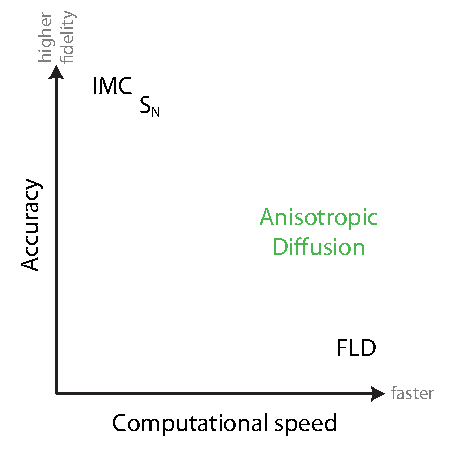
\includegraphics[width=2in]{../figures/fidelity2}
  \end{center}
{\setlength{\baselineskip}{-\baselineskip} \tiny 
This material is based upon work supported under a National Science Foundation
Graduate Research Fellowship and a Department of Energy Nuclear Energy
University Programs Graduate Fellowship. Any opinions, findings, conclusions or
recommendations expressed in this publication are those of the author and do
not necessarily reflect the views of the National Science Foundation or the
Department of Energy Office of Nuclear Energy.\par}
\end{frame}

%%%%%%%%%%%%%%%%%%%%%%%%%%%%%%%%%%%%%%%%
\begin{frame}
  \frametitle{References}
\bibliographystyle{ans}
\bibliography{../SRJall}
\end{frame}
%%%%%%%%%%%%%%%%%%%%%%%%%%%%%%%%%%%%%%%%%%%%%%%%%%%%%%%%%%%%%%%%%%%%%%%%%%%

%	This material is based upon work supported under a National Science
%	Foundation Graduate Research Fellowship. Any opinions, findings, conclusions
%	or recommendations expressed in this publication are those of the author(s)
%	and do not necessarily reflect the views of the National Science
%	Foundation.  
\end{document}
